\documentclass{standalone}
\usepackage{tikz}
\usetikzlibrary{patterns}
\usetikzlibrary{positioning}
\usetikzlibrary{patterns, positioning}
\usetikzlibrary{shapes.misc}
\usepackage[outline]{contour}
\contourlength{1.5pt} 
\usetikzlibrary{calc}
        \usepackage{relsize}
        \tikzset{fontscale/.style = {font=\relsize{#1}}}

\begin{document}
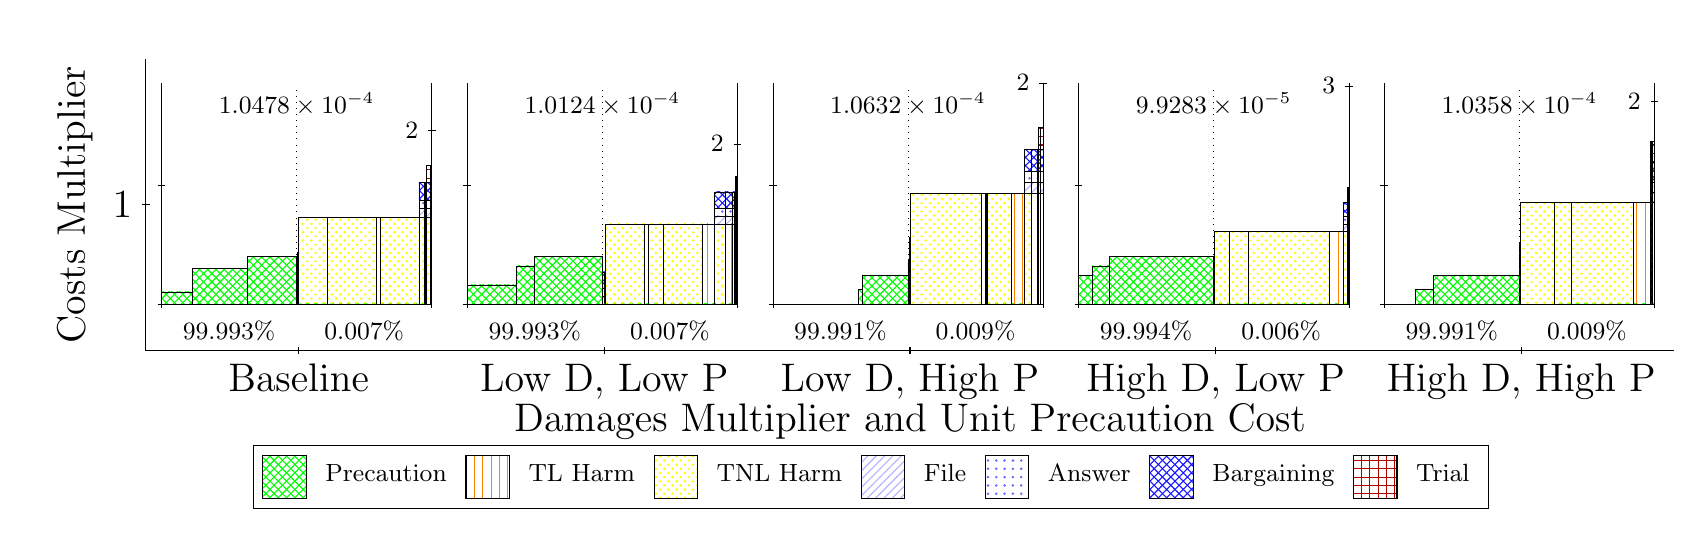
\begin{tikzpicture}
\clip(-0.5,-1.1) rectangle +(20.91,6.2);
\draw[black] (1,1) -- (1,4.7);
\node[rotate=90, fontscale=2, anchor=center] at (0.1, 2.85) {Costs Multiplier};
\draw[black] (0.95,2.85) -- (1.05,2.85);
\node[fontscale=2, anchor=east] at (0.95, 2.85) {1};

\draw[black] (1,1) -- (20.41,1);
\node[fontscale=2, anchor=center] at (10.705, 0.1) {Damages Multiplier and Unit Precaution Cost};
\draw[black] (2.941,0.95) -- (2.941,1.05);
\node[fontscale=2, anchor=north] at (2.941, 0.95) {Baseline};
\draw[black] (6.823,0.95) -- (6.823,1.05);
\node[fontscale=2, anchor=north] at (6.823, 0.95) {Low D, Low P};
\draw[black] (10.705,0.95) -- (10.705,1.05);
\node[fontscale=2, anchor=north] at (10.705, 0.95) {Low D, High P};
\draw[black] (14.587,0.95) -- (14.587,1.05);
\node[fontscale=2, anchor=north] at (14.587, 0.95) {High D, Low P};
\draw[black] (18.469,0.95) -- (18.469,1.05);
\node[fontscale=2, anchor=north] at (18.469, 0.95) {High D, High P};


\draw[pattern=crosshatch, pattern color=green,draw=black,very thin] (1.2,1.592) rectangle (1.5947,1.7431);
\draw[pattern=crosshatch, pattern color=green,draw=black,very thin] (1.5947,1.592) rectangle (2.2894,2.0454);
\draw[pattern=crosshatch, pattern color=green,draw=black,very thin] (2.2894,1.592) rectangle (2.916,2.1965);
\draw[pattern=crosshatch, pattern color=green,draw=black,very thin] (2.916,1.592) rectangle (2.9243,1.592);
\draw[pattern=north east lines, pattern color=blue!30,draw=black,very thin] (2.916,1.592) rectangle (2.9243,1.702);
\draw[pattern=dots,  pattern color=blue!60,draw=black,very thin] (2.916,1.702) rectangle (2.9243,1.812);
\draw[pattern=crosshatch,      pattern color=blue!90,draw=black,very thin] (2.916,1.812) rectangle (2.9243,2.032);
\draw[pattern=crosshatch, pattern color=green,draw=black,very thin] (2.9243,1.592) rectangle (2.9274,1.592);
\draw[pattern=north east lines, pattern color=blue!30,draw=black,very thin] (2.9243,1.592) rectangle (2.9274,1.702);
\draw[pattern=dots,  pattern color=blue!60,draw=black,very thin] (2.9243,1.702) rectangle (2.9274,1.812);
\draw[pattern=crosshatch,      pattern color=blue!90,draw=black,very thin] (2.9243,1.812) rectangle (2.9274,2.032);
\draw[pattern=crosshatch, pattern color=green,draw=black,very thin] (2.9274,1.592) rectangle (2.9334,1.592);
\draw[pattern=north east lines, pattern color=blue!30,draw=black,very thin] (2.9274,1.592) rectangle (2.9334,1.702);
\draw[pattern=dots,  pattern color=blue!60,draw=black,very thin] (2.9274,1.702) rectangle (2.9334,1.812);
\draw[pattern=crosshatch,      pattern color=blue!90,draw=black,very thin] (2.9274,1.812) rectangle (2.9334,2.032);
\draw[pattern=grid,            pattern color=red!70!black,draw=black,very thin] (2.9274,2.032) rectangle (2.9334,2.252);
\draw[pattern=crosshatch, pattern color=green,draw=black,very thin] (2.9334,1.592) rectangle (2.9354,1.592);
\draw[pattern=north east lines, pattern color=blue!30,draw=black,very thin] (2.9334,1.592) rectangle (2.9354,1.702);
\draw[pattern=dots,  pattern color=blue!60,draw=black,very thin] (2.9334,1.702) rectangle (2.9354,1.812);
\draw[pattern=crosshatch,      pattern color=blue!90,draw=black,very thin] (2.9334,1.812) rectangle (2.9354,2.032);
\draw[pattern=grid,            pattern color=red!70!black,draw=black,very thin] (2.9334,2.032) rectangle (2.9354,2.252);
\draw[pattern=crosshatch, pattern color=green,draw=black,very thin] (2.9354,1.592) rectangle (3.3039,1.592);
\draw[pattern=crosshatch dots, pattern color=yellow,draw=black,very thin] (2.9354,1.592) rectangle (3.3039,2.692);
\draw[pattern=crosshatch, pattern color=green,draw=black,very thin] (3.3039,1.592) rectangle (3.3061,1.592);
\draw[pattern=vertical lines, pattern color=orange,draw=black,very thin] (3.3039,1.592) rectangle (3.3061,2.692);
\draw[pattern=crosshatch, pattern color=green,draw=black,very thin] (3.3061,1.592) rectangle (3.9318,1.592);
\draw[pattern=crosshatch dots, pattern color=yellow,draw=black,very thin] (3.3061,1.592) rectangle (3.9318,2.692);
\draw[pattern=crosshatch, pattern color=green,draw=black,very thin] (3.9318,1.592) rectangle (3.977,1.592);
\draw[pattern=vertical lines, pattern color=orange,draw=black,very thin] (3.9318,1.592) rectangle (3.977,2.692);
\draw[pattern=crosshatch, pattern color=green,draw=black,very thin] (3.977,1.592) rectangle (4.4677,1.592);
\draw[pattern=crosshatch dots, pattern color=yellow,draw=black,very thin] (3.977,1.592) rectangle (4.4677,2.692);
\draw[pattern=crosshatch, pattern color=green,draw=black,very thin] (4.4677,1.592) rectangle (4.5339,1.592);
\draw[pattern=crosshatch dots, pattern color=yellow,draw=black,very thin] (4.4677,1.592) rectangle (4.5339,2.692);
\draw[pattern=north east lines, pattern color=blue!30,draw=black,very thin] (4.4677,2.692) rectangle (4.5339,2.802);
\draw[pattern=dots,  pattern color=blue!60,draw=black,very thin] (4.4677,2.802) rectangle (4.5339,2.912);
\draw[pattern=crosshatch,      pattern color=blue!90,draw=black,very thin] (4.4677,2.912) rectangle (4.5339,3.132);
\draw[pattern=crosshatch, pattern color=green,draw=black,very thin] (4.5339,1.592) rectangle (4.5435,1.592);
\draw[pattern=vertical lines, pattern color=orange,draw=black,very thin] (4.5339,1.592) rectangle (4.5435,2.692);
\draw[pattern=north east lines, pattern color=blue!30,draw=black,very thin] (4.5339,2.692) rectangle (4.5435,2.802);
\draw[pattern=dots,  pattern color=blue!60,draw=black,very thin] (4.5339,2.802) rectangle (4.5435,2.912);
\draw[pattern=crosshatch,      pattern color=blue!90,draw=black,very thin] (4.5339,2.912) rectangle (4.5435,3.132);
\draw[pattern=crosshatch, pattern color=green,draw=black,very thin] (4.5435,1.592) rectangle (4.5503,1.592);
\draw[pattern=crosshatch dots, pattern color=yellow,draw=black,very thin] (4.5435,1.592) rectangle (4.5503,2.692);
\draw[pattern=north east lines, pattern color=blue!30,draw=black,very thin] (4.5435,2.692) rectangle (4.5503,2.802);
\draw[pattern=dots,  pattern color=blue!60,draw=black,very thin] (4.5435,2.802) rectangle (4.5503,2.912);
\draw[pattern=crosshatch,      pattern color=blue!90,draw=black,very thin] (4.5435,2.912) rectangle (4.5503,3.132);
\draw[pattern=crosshatch, pattern color=green,draw=black,very thin] (4.5503,1.592) rectangle (4.5634,1.592);
\draw[pattern=vertical lines, pattern color=orange,draw=black,very thin] (4.5503,1.592) rectangle (4.5634,2.692);
\draw[pattern=north east lines, pattern color=blue!30,draw=black,very thin] (4.5503,2.692) rectangle (4.5634,2.802);
\draw[pattern=dots,  pattern color=blue!60,draw=black,very thin] (4.5503,2.802) rectangle (4.5634,2.912);
\draw[pattern=crosshatch,      pattern color=blue!90,draw=black,very thin] (4.5503,2.912) rectangle (4.5634,3.132);
\draw[pattern=crosshatch, pattern color=green,draw=black,very thin] (4.5634,1.592) rectangle (4.612,1.592);
\draw[pattern=crosshatch dots, pattern color=yellow,draw=black,very thin] (4.5634,1.592) rectangle (4.612,2.692);
\draw[pattern=north east lines, pattern color=blue!30,draw=black,very thin] (4.5634,2.692) rectangle (4.612,2.802);
\draw[pattern=dots,  pattern color=blue!60,draw=black,very thin] (4.5634,2.802) rectangle (4.612,2.912);
\draw[pattern=crosshatch,      pattern color=blue!90,draw=black,very thin] (4.5634,2.912) rectangle (4.612,3.132);
\draw[pattern=grid,            pattern color=red!70!black,draw=black,very thin] (4.5634,3.132) rectangle (4.612,3.352);
\draw[pattern=crosshatch, pattern color=green,draw=black,very thin] (4.612,1.592) rectangle (4.6185,1.592);
\draw[pattern=vertical lines, pattern color=orange,draw=black,very thin] (4.612,1.592) rectangle (4.6185,2.692);
\draw[pattern=north east lines, pattern color=blue!30,draw=black,very thin] (4.612,2.692) rectangle (4.6185,2.802);
\draw[pattern=dots,  pattern color=blue!60,draw=black,very thin] (4.612,2.802) rectangle (4.6185,2.912);
\draw[pattern=crosshatch,      pattern color=blue!90,draw=black,very thin] (4.612,2.912) rectangle (4.6185,3.132);
\draw[pattern=grid,            pattern color=red!70!black,draw=black,very thin] (4.612,3.132) rectangle (4.6185,3.352);
\draw[pattern=crosshatch, pattern color=green,draw=black,very thin] (4.6185,1.592) rectangle (4.6264,1.592);
\draw[pattern=crosshatch dots, pattern color=yellow,draw=black,very thin] (4.6185,1.592) rectangle (4.6264,2.692);
\draw[pattern=north east lines, pattern color=blue!30,draw=black,very thin] (4.6185,2.692) rectangle (4.6264,2.802);
\draw[pattern=dots,  pattern color=blue!60,draw=black,very thin] (4.6185,2.802) rectangle (4.6264,2.912);
\draw[pattern=crosshatch,      pattern color=blue!90,draw=black,very thin] (4.6185,2.912) rectangle (4.6264,3.132);
\draw[pattern=grid,            pattern color=red!70!black,draw=black,very thin] (4.6185,3.132) rectangle (4.6264,3.352);
\draw[pattern=crosshatch, pattern color=green,draw=black,very thin] (4.6264,1.592) rectangle (4.632,1.592);
\draw[pattern=vertical lines, pattern color=orange,draw=black,very thin] (4.6264,1.592) rectangle (4.632,2.692);
\draw[pattern=north east lines, pattern color=blue!30,draw=black,very thin] (4.6264,2.692) rectangle (4.632,2.802);
\draw[pattern=dots,  pattern color=blue!60,draw=black,very thin] (4.6264,2.802) rectangle (4.632,2.912);
\draw[pattern=crosshatch,      pattern color=blue!90,draw=black,very thin] (4.6264,2.912) rectangle (4.632,3.132);
\draw[pattern=grid,            pattern color=red!70!black,draw=black,very thin] (4.6264,3.132) rectangle (4.632,3.352);
\node[font=\small,text=black,anchor=north] at (2.916, 4.4) {$1.0478\times 10^{-4}$};
\draw[black,very thin] (1.2,1.592) -- (1.2,4.4);
\draw[black,very thin] (1.15,1.592) -- (1.25,1.592);
\node[font=\small,text=black, anchor=west] at (1.15, 1.592) {};
\draw[black,very thin] (1.15,3.1032) -- (1.25,3.1032);
\node[font=\small,text=black, anchor=west] at (1.15, 3.1032) {};

\draw[black,dotted,very thin] (2.916,1.6762) -- (2.916,4.3158);
\draw[black,very thin] (4.632,1.592) -- (4.632,4.4);
\draw[black,very thin] (4.582,3.7919) -- (4.682,3.7919);
\node[font=\small,text=black, anchor=east] at (4.582, 3.7919) {\contour{white}{2}};

\draw[black,very thin] (1.2,1.592) -- (4.632,1.592);
\draw[black,very thin] (1.2,1.542) -- (1.2,1.642);
\node[font=\small,text=black, anchor=north] at (1.2, 1.542) {};
\draw[black,very thin] (4.632,1.542) -- (4.632,1.642);
\node[font=\small,text=black, anchor=north] at (4.632, 1.542) {};

\node[font=\small,text=black,anchor=south] at (2.058, 0.992) {99.993\%};
\node[font=\small,text=black,anchor=south] at (3.774, 0.992) {0.007\%};

\draw[pattern=crosshatch, pattern color=green,draw=black,very thin] (5.082,1.592) rectangle (5.7085,1.8338);
\draw[pattern=crosshatch, pattern color=green,draw=black,very thin] (5.7085,1.592) rectangle (5.94,2.0756);
\draw[pattern=crosshatch, pattern color=green,draw=black,very thin] (5.94,1.592) rectangle (6.798,2.1965);
\draw[pattern=crosshatch, pattern color=green,draw=black,very thin] (6.798,1.592) rectangle (6.8253,1.592);
\draw[pattern=north east lines, pattern color=blue!30,draw=black,very thin] (6.798,1.592) rectangle (6.8253,1.6936);
\draw[pattern=dots,  pattern color=blue!60,draw=black,very thin] (6.798,1.6936) rectangle (6.8253,1.7951);
\draw[pattern=crosshatch,      pattern color=blue!90,draw=black,very thin] (6.798,1.7951) rectangle (6.8253,1.9982);
\draw[pattern=crosshatch, pattern color=green,draw=black,very thin] (6.8253,1.592) rectangle (6.8317,1.592);
\draw[pattern=north east lines, pattern color=blue!30,draw=black,very thin] (6.8253,1.592) rectangle (6.8317,1.6936);
\draw[pattern=dots,  pattern color=blue!60,draw=black,very thin] (6.8253,1.6936) rectangle (6.8317,1.7951);
\draw[pattern=crosshatch,      pattern color=blue!90,draw=black,very thin] (6.8253,1.7951) rectangle (6.8317,1.9983);
\draw[pattern=crosshatch, pattern color=green,draw=black,very thin] (6.8317,1.592) rectangle (6.8347,1.592);
\draw[pattern=north east lines, pattern color=blue!30,draw=black,very thin] (6.8317,1.592) rectangle (6.8347,1.6936);
\draw[pattern=dots,  pattern color=blue!60,draw=black,very thin] (6.8317,1.6936) rectangle (6.8347,1.7951);
\draw[pattern=crosshatch,      pattern color=blue!90,draw=black,very thin] (6.8317,1.7951) rectangle (6.8347,1.9982);
\draw[pattern=grid,            pattern color=red!70!black,draw=black,very thin] (6.8317,1.9982) rectangle (6.8347,2.2014);
\draw[pattern=crosshatch, pattern color=green,draw=black,very thin] (6.8347,1.592) rectangle (7.3369,1.592);
\draw[pattern=crosshatch dots, pattern color=yellow,draw=black,very thin] (6.8347,1.592) rectangle (7.3369,2.6076);
\draw[pattern=crosshatch, pattern color=green,draw=black,very thin] (7.3369,1.592) rectangle (7.3772,1.592);
\draw[pattern=vertical lines, pattern color=orange,draw=black,very thin] (7.3369,1.592) rectangle (7.3772,2.6076);
\draw[pattern=crosshatch, pattern color=green,draw=black,very thin] (7.3772,1.592) rectangle (7.5659,1.592);
\draw[pattern=crosshatch dots, pattern color=yellow,draw=black,very thin] (7.3772,1.592) rectangle (7.5659,2.6076);
\draw[pattern=crosshatch, pattern color=green,draw=black,very thin] (7.5659,1.592) rectangle (7.57,1.592);
\draw[pattern=vertical lines, pattern color=orange,draw=black,very thin] (7.5659,1.592) rectangle (7.57,2.6076);
\draw[pattern=crosshatch, pattern color=green,draw=black,very thin] (7.57,1.592) rectangle (8.064,1.592);
\draw[pattern=crosshatch dots, pattern color=yellow,draw=black,very thin] (7.57,1.592) rectangle (8.064,2.6076);
\draw[pattern=crosshatch, pattern color=green,draw=black,very thin] (8.064,1.592) rectangle (8.2248,1.592);
\draw[pattern=vertical lines, pattern color=orange,draw=black,very thin] (8.064,1.592) rectangle (8.2248,2.6076);
\draw[pattern=crosshatch, pattern color=green,draw=black,very thin] (8.2248,1.592) rectangle (8.3557,1.592);
\draw[pattern=crosshatch dots, pattern color=yellow,draw=black,very thin] (8.2248,1.592) rectangle (8.3557,2.6076);
\draw[pattern=north east lines, pattern color=blue!30,draw=black,very thin] (8.2248,2.6076) rectangle (8.3557,2.7091);
\draw[pattern=dots,  pattern color=blue!60,draw=black,very thin] (8.2248,2.7091) rectangle (8.3557,2.8107);
\draw[pattern=crosshatch,      pattern color=blue!90,draw=black,very thin] (8.2248,2.8107) rectangle (8.3557,3.0138);
\draw[pattern=crosshatch, pattern color=green,draw=black,very thin] (8.3557,1.592) rectangle (8.4513,1.592);
\draw[pattern=vertical lines, pattern color=orange,draw=black,very thin] (8.3557,1.592) rectangle (8.4513,2.6076);
\draw[pattern=north east lines, pattern color=blue!30,draw=black,very thin] (8.3557,2.6076) rectangle (8.4513,2.7091);
\draw[pattern=dots,  pattern color=blue!60,draw=black,very thin] (8.3557,2.7091) rectangle (8.4513,2.8107);
\draw[pattern=crosshatch,      pattern color=blue!90,draw=black,very thin] (8.3557,2.8107) rectangle (8.4513,3.0138);
\draw[pattern=crosshatch, pattern color=green,draw=black,very thin] (8.4513,1.592) rectangle (8.48,1.592);
\draw[pattern=crosshatch dots, pattern color=yellow,draw=black,very thin] (8.4513,1.592) rectangle (8.48,2.6076);
\draw[pattern=north east lines, pattern color=blue!30,draw=black,very thin] (8.4513,2.6076) rectangle (8.48,2.7092);
\draw[pattern=dots,  pattern color=blue!60,draw=black,very thin] (8.4513,2.7092) rectangle (8.48,2.8107);
\draw[pattern=crosshatch,      pattern color=blue!90,draw=black,very thin] (8.4513,2.8107) rectangle (8.48,3.0138);
\draw[pattern=crosshatch, pattern color=green,draw=black,very thin] (8.48,1.592) rectangle (8.49,1.592);
\draw[pattern=vertical lines, pattern color=orange,draw=black,very thin] (8.48,1.592) rectangle (8.49,2.6076);
\draw[pattern=north east lines, pattern color=blue!30,draw=black,very thin] (8.48,2.6076) rectangle (8.49,2.7092);
\draw[pattern=dots,  pattern color=blue!60,draw=black,very thin] (8.48,2.7092) rectangle (8.49,2.8107);
\draw[pattern=crosshatch,      pattern color=blue!90,draw=black,very thin] (8.48,2.8107) rectangle (8.49,3.0138);
\draw[pattern=crosshatch, pattern color=green,draw=black,very thin] (8.49,1.592) rectangle (8.4929,1.592);
\draw[pattern=crosshatch dots, pattern color=yellow,draw=black,very thin] (8.49,1.592) rectangle (8.4929,2.6076);
\draw[pattern=north east lines, pattern color=blue!30,draw=black,very thin] (8.49,2.6076) rectangle (8.4929,2.7091);
\draw[pattern=dots,  pattern color=blue!60,draw=black,very thin] (8.49,2.7091) rectangle (8.4929,2.8107);
\draw[pattern=crosshatch,      pattern color=blue!90,draw=black,very thin] (8.49,2.8107) rectangle (8.4929,3.0138);
\draw[pattern=grid,            pattern color=red!70!black,draw=black,very thin] (8.49,3.0138) rectangle (8.4929,3.2169);
\draw[pattern=crosshatch, pattern color=green,draw=black,very thin] (8.4929,1.592) rectangle (8.514,1.592);
\draw[pattern=vertical lines, pattern color=orange,draw=black,very thin] (8.4929,1.592) rectangle (8.514,2.6076);
\draw[pattern=north east lines, pattern color=blue!30,draw=black,very thin] (8.4929,2.6076) rectangle (8.514,2.7091);
\draw[pattern=dots,  pattern color=blue!60,draw=black,very thin] (8.4929,2.7091) rectangle (8.514,2.8107);
\draw[pattern=crosshatch,      pattern color=blue!90,draw=black,very thin] (8.4929,2.8107) rectangle (8.514,3.0138);
\draw[pattern=grid,            pattern color=red!70!black,draw=black,very thin] (8.4929,3.0138) rectangle (8.514,3.2169);
\node[font=\small,text=black,anchor=north] at (6.798, 4.4) {$1.0124\times 10^{-4}$};
\draw[black,very thin] (5.082,1.592) -- (5.082,4.4);
\draw[black,very thin] (5.032,1.592) -- (5.132,1.592);
\node[font=\small,text=black, anchor=west] at (5.032, 1.592) {};
\draw[black,very thin] (5.032,3.1032) -- (5.132,3.1032);
\node[font=\small,text=black, anchor=west] at (5.032, 3.1032) {};

\draw[black,dotted,very thin] (6.798,1.6762) -- (6.798,4.3158);
\draw[black,very thin] (8.514,1.592) -- (8.514,4.4);
\draw[black,very thin] (8.464,3.6231) -- (8.564,3.6231);
\node[font=\small,text=black, anchor=east] at (8.464, 3.6231) {\contour{white}{2}};

\draw[black,very thin] (5.082,1.592) -- (8.514,1.592);
\draw[black,very thin] (5.082,1.542) -- (5.082,1.642);
\node[font=\small,text=black, anchor=north] at (5.082, 1.542) {};
\draw[black,very thin] (8.514,1.542) -- (8.514,1.642);
\node[font=\small,text=black, anchor=north] at (8.514, 1.542) {};

\node[font=\small,text=black,anchor=south] at (5.94, 0.992) {99.993\%};
\node[font=\small,text=black,anchor=south] at (7.656, 0.992) {0.007\%};

\draw[pattern=crosshatch, pattern color=green,draw=black,very thin] (10.053,1.592) rectangle (10.101,1.7733);
\draw[pattern=crosshatch, pattern color=green,draw=black,very thin] (10.101,1.592) rectangle (10.68,1.9547);
\draw[pattern=north east lines, pattern color=blue!30,draw=black,very thin] (10.68,1.592) rectangle (10.696,1.7324);
\draw[pattern=dots,  pattern color=blue!60,draw=black,very thin] (10.68,1.7324) rectangle (10.696,1.8728);
\draw[pattern=crosshatch,      pattern color=blue!90,draw=black,very thin] (10.68,1.8728) rectangle (10.696,2.1536);
\draw[pattern=crosshatch, pattern color=green,draw=black,very thin] (10.696,1.592) rectangle (10.698,1.592);
\draw[pattern=north east lines, pattern color=blue!30,draw=black,very thin] (10.696,1.592) rectangle (10.698,1.7324);
\draw[pattern=dots,  pattern color=blue!60,draw=black,very thin] (10.696,1.7324) rectangle (10.698,1.8728);
\draw[pattern=crosshatch,      pattern color=blue!90,draw=black,very thin] (10.696,1.8728) rectangle (10.698,2.1536);
\draw[pattern=north east lines, pattern color=blue!30,draw=black,very thin] (10.698,1.592) rectangle (10.704,1.7324);
\draw[pattern=dots,  pattern color=blue!60,draw=black,very thin] (10.698,1.7324) rectangle (10.704,1.8728);
\draw[pattern=crosshatch,      pattern color=blue!90,draw=black,very thin] (10.698,1.8728) rectangle (10.704,2.1536);
\draw[pattern=grid,            pattern color=red!70!black,draw=black,very thin] (10.698,2.1536) rectangle (10.704,2.4344);
\draw[pattern=crosshatch dots, pattern color=yellow,draw=black,very thin] (10.704,1.592) rectangle (11.609,2.996);
\draw[pattern=vertical lines, pattern color=orange,draw=black,very thin] (11.609,1.592) rectangle (11.657,2.996);
\draw[pattern=crosshatch, pattern color=green,draw=black,very thin] (11.657,1.592) rectangle (11.679,1.592);
\draw[pattern=crosshatch dots, pattern color=yellow,draw=black,very thin] (11.657,1.592) rectangle (11.679,2.996);
\draw[pattern=crosshatch, pattern color=green,draw=black,very thin] (11.679,1.592) rectangle (11.687,1.592);
\draw[pattern=vertical lines, pattern color=orange,draw=black,very thin] (11.679,1.592) rectangle (11.687,2.996);
\draw[pattern=crosshatch, pattern color=green,draw=black,very thin] (11.687,1.592) rectangle (11.996,1.592);
\draw[pattern=crosshatch dots, pattern color=yellow,draw=black,very thin] (11.687,1.592) rectangle (11.996,2.996);
\draw[pattern=crosshatch, pattern color=green,draw=black,very thin] (11.996,1.592) rectangle (12.161,1.592);
\draw[pattern=vertical lines, pattern color=orange,draw=black,very thin] (11.996,1.592) rectangle (12.161,2.996);
\draw[pattern=crosshatch dots, pattern color=yellow,draw=black,very thin] (12.161,1.592) rectangle (12.244,2.996);
\draw[pattern=north east lines, pattern color=blue!30,draw=black,very thin] (12.161,2.996) rectangle (12.244,3.1364);
\draw[pattern=dots,  pattern color=blue!60,draw=black,very thin] (12.161,3.1364) rectangle (12.244,3.2768);
\draw[pattern=crosshatch,      pattern color=blue!90,draw=black,very thin] (12.161,3.2768) rectangle (12.244,3.5576);
\draw[pattern=vertical lines, pattern color=orange,draw=black,very thin] (12.244,1.592) rectangle (12.324,2.996);
\draw[pattern=north east lines, pattern color=blue!30,draw=black,very thin] (12.244,2.996) rectangle (12.324,3.1364);
\draw[pattern=dots,  pattern color=blue!60,draw=black,very thin] (12.244,3.1364) rectangle (12.324,3.2768);
\draw[pattern=crosshatch,      pattern color=blue!90,draw=black,very thin] (12.244,3.2768) rectangle (12.324,3.5576);
\draw[pattern=crosshatch, pattern color=green,draw=black,very thin] (12.324,1.592) rectangle (12.328,1.592);
\draw[pattern=crosshatch dots, pattern color=yellow,draw=black,very thin] (12.324,1.592) rectangle (12.328,2.996);
\draw[pattern=north east lines, pattern color=blue!30,draw=black,very thin] (12.324,2.996) rectangle (12.328,3.1364);
\draw[pattern=dots,  pattern color=blue!60,draw=black,very thin] (12.324,3.1364) rectangle (12.328,3.2768);
\draw[pattern=crosshatch,      pattern color=blue!90,draw=black,very thin] (12.324,3.2768) rectangle (12.328,3.5576);
\draw[pattern=crosshatch, pattern color=green,draw=black,very thin] (12.328,1.592) rectangle (12.339,1.592);
\draw[pattern=vertical lines, pattern color=orange,draw=black,very thin] (12.328,1.592) rectangle (12.339,2.996);
\draw[pattern=north east lines, pattern color=blue!30,draw=black,very thin] (12.328,2.996) rectangle (12.339,3.1364);
\draw[pattern=dots,  pattern color=blue!60,draw=black,very thin] (12.328,3.1364) rectangle (12.339,3.2768);
\draw[pattern=crosshatch,      pattern color=blue!90,draw=black,very thin] (12.328,3.2768) rectangle (12.339,3.5576);
\draw[pattern=crosshatch dots, pattern color=yellow,draw=black,very thin] (12.339,1.592) rectangle (12.359,2.996);
\draw[pattern=north east lines, pattern color=blue!30,draw=black,very thin] (12.339,2.996) rectangle (12.359,3.1364);
\draw[pattern=dots,  pattern color=blue!60,draw=black,very thin] (12.339,3.1364) rectangle (12.359,3.2768);
\draw[pattern=crosshatch,      pattern color=blue!90,draw=black,very thin] (12.339,3.2768) rectangle (12.359,3.5576);
\draw[pattern=grid,            pattern color=red!70!black,draw=black,very thin] (12.339,3.5576) rectangle (12.359,3.8384);
\draw[pattern=vertical lines, pattern color=orange,draw=black,very thin] (12.359,1.592) rectangle (12.396,2.996);
\draw[pattern=north east lines, pattern color=blue!30,draw=black,very thin] (12.359,2.996) rectangle (12.396,3.1364);
\draw[pattern=dots,  pattern color=blue!60,draw=black,very thin] (12.359,3.1364) rectangle (12.396,3.2768);
\draw[pattern=crosshatch,      pattern color=blue!90,draw=black,very thin] (12.359,3.2768) rectangle (12.396,3.5576);
\draw[pattern=grid,            pattern color=red!70!black,draw=black,very thin] (12.359,3.5576) rectangle (12.396,3.8384);
\node[font=\small,text=black,anchor=north] at (10.68, 4.4) {$1.0632\times 10^{-4}$};
\draw[black,very thin] (8.964,1.592) -- (8.964,4.4);
\draw[black,very thin] (8.914,1.592) -- (9.014,1.592);
\node[font=\small,text=black, anchor=west] at (8.914, 1.592) {};
\draw[black,very thin] (8.914,3.1031) -- (9.014,3.1031);
\node[font=\small,text=black, anchor=west] at (8.914, 3.1031) {};

\draw[black,dotted,very thin] (10.68,1.6762) -- (10.68,4.3158);
\draw[black,very thin] (12.396,1.592) -- (12.396,4.4);
\draw[black,very thin] (12.346,4.4) -- (12.446,4.4);
\node[font=\small,text=black, anchor=east] at (12.346, 4.4) {\contour{white}{2}};

\draw[black,very thin] (8.964,1.592) -- (12.396,1.592);
\draw[black,very thin] (8.964,1.542) -- (8.964,1.642);
\node[font=\small,text=black, anchor=north] at (8.964, 1.542) {};
\draw[black,very thin] (12.396,1.542) -- (12.396,1.642);
\node[font=\small,text=black, anchor=north] at (12.396, 1.542) {};

\node[font=\small,text=black,anchor=south] at (9.822, 0.992) {99.991\%};
\node[font=\small,text=black,anchor=south] at (11.538, 0.992) {0.009\%};

\draw[pattern=crosshatch, pattern color=green,draw=black,very thin] (12.846,1.592) rectangle (13.022,1.9547);
\draw[pattern=crosshatch, pattern color=green,draw=black,very thin] (13.022,1.592) rectangle (13.241,2.0756);
\draw[pattern=crosshatch, pattern color=green,draw=black,very thin] (13.241,1.592) rectangle (14.562,2.1965);
\draw[pattern=crosshatch, pattern color=green,draw=black,very thin] (14.562,1.592) rectangle (14.568,1.592);
\draw[pattern=north east lines, pattern color=blue!30,draw=black,very thin] (14.562,1.592) rectangle (14.568,1.6843);
\draw[pattern=dots,  pattern color=blue!60,draw=black,very thin] (14.562,1.6843) rectangle (14.568,1.7766);
\draw[pattern=crosshatch,      pattern color=blue!90,draw=black,very thin] (14.562,1.7766) rectangle (14.568,1.9611);
\draw[pattern=crosshatch, pattern color=green,draw=black,very thin] (14.568,1.592) rectangle (14.57,1.592);
\draw[pattern=north east lines, pattern color=blue!30,draw=black,very thin] (14.568,1.592) rectangle (14.57,1.6843);
\draw[pattern=dots,  pattern color=blue!60,draw=black,very thin] (14.568,1.6843) rectangle (14.57,1.7766);
\draw[pattern=crosshatch,      pattern color=blue!90,draw=black,very thin] (14.568,1.7766) rectangle (14.57,1.9611);
\draw[pattern=grid,            pattern color=red!70!black,draw=black,very thin] (14.568,1.9611) rectangle (14.57,2.1457);
\draw[pattern=crosshatch, pattern color=green,draw=black,very thin] (14.57,1.592) rectangle (14.755,1.592);
\draw[pattern=crosshatch dots, pattern color=yellow,draw=black,very thin] (14.57,1.592) rectangle (14.755,2.5147);
\draw[pattern=crosshatch, pattern color=green,draw=black,very thin] (14.755,1.592) rectangle (14.755,1.592);
\draw[pattern=vertical lines, pattern color=orange,draw=black,very thin] (14.755,1.592) rectangle (14.755,2.5147);
\draw[pattern=crosshatch, pattern color=green,draw=black,very thin] (14.755,1.592) rectangle (15.005,1.592);
\draw[pattern=crosshatch dots, pattern color=yellow,draw=black,very thin] (14.755,1.592) rectangle (15.005,2.5147);
\draw[pattern=crosshatch, pattern color=green,draw=black,very thin] (15.005,1.592) rectangle (16.032,1.592);
\draw[pattern=crosshatch dots, pattern color=yellow,draw=black,very thin] (15.005,1.592) rectangle (16.032,2.5148);
\draw[pattern=crosshatch, pattern color=green,draw=black,very thin] (16.032,1.592) rectangle (16.213,1.592);
\draw[pattern=vertical lines, pattern color=orange,draw=black,very thin] (16.032,1.592) rectangle (16.213,2.5148);
\draw[pattern=crosshatch, pattern color=green,draw=black,very thin] (16.213,1.592) rectangle (16.258,1.592);
\draw[pattern=crosshatch dots, pattern color=yellow,draw=black,very thin] (16.213,1.592) rectangle (16.258,2.5147);
\draw[pattern=north east lines, pattern color=blue!30,draw=black,very thin] (16.213,2.5147) rectangle (16.258,2.607);
\draw[pattern=dots,  pattern color=blue!60,draw=black,very thin] (16.213,2.607) rectangle (16.258,2.6993);
\draw[pattern=crosshatch,      pattern color=blue!90,draw=black,very thin] (16.213,2.6993) rectangle (16.258,2.8838);
\draw[pattern=crosshatch, pattern color=green,draw=black,very thin] (16.258,1.592) rectangle (16.26,1.592);
\draw[pattern=vertical lines, pattern color=orange,draw=black,very thin] (16.258,1.592) rectangle (16.26,2.5147);
\draw[pattern=north east lines, pattern color=blue!30,draw=black,very thin] (16.258,2.5147) rectangle (16.26,2.607);
\draw[pattern=dots,  pattern color=blue!60,draw=black,very thin] (16.258,2.607) rectangle (16.26,2.6993);
\draw[pattern=crosshatch,      pattern color=blue!90,draw=black,very thin] (16.258,2.6993) rectangle (16.26,2.8838);
\draw[pattern=crosshatch, pattern color=green,draw=black,very thin] (16.26,1.592) rectangle (16.262,1.592);
\draw[pattern=crosshatch dots, pattern color=yellow,draw=black,very thin] (16.26,1.592) rectangle (16.262,2.5147);
\draw[pattern=north east lines, pattern color=blue!30,draw=black,very thin] (16.26,2.5147) rectangle (16.262,2.607);
\draw[pattern=dots,  pattern color=blue!60,draw=black,very thin] (16.26,2.607) rectangle (16.262,2.6993);
\draw[pattern=crosshatch,      pattern color=blue!90,draw=black,very thin] (16.26,2.6993) rectangle (16.262,2.8838);
\draw[pattern=grid,            pattern color=red!70!black,draw=black,very thin] (16.26,2.8838) rectangle (16.262,3.0684);
\draw[pattern=crosshatch, pattern color=green,draw=black,very thin] (16.262,1.592) rectangle (16.262,1.592);
\draw[pattern=vertical lines, pattern color=orange,draw=black,very thin] (16.262,1.592) rectangle (16.262,2.5147);
\draw[pattern=north east lines, pattern color=blue!30,draw=black,very thin] (16.262,2.5147) rectangle (16.262,2.607);
\draw[pattern=dots,  pattern color=blue!60,draw=black,very thin] (16.262,2.607) rectangle (16.262,2.6993);
\draw[pattern=crosshatch,      pattern color=blue!90,draw=black,very thin] (16.262,2.6993) rectangle (16.262,2.8838);
\draw[pattern=grid,            pattern color=red!70!black,draw=black,very thin] (16.262,2.8838) rectangle (16.262,3.0684);
\draw[pattern=crosshatch, pattern color=green,draw=black,very thin] (16.262,1.592) rectangle (16.277,1.592);
\draw[pattern=crosshatch dots, pattern color=yellow,draw=black,very thin] (16.262,1.592) rectangle (16.277,2.5147);
\draw[pattern=north east lines, pattern color=blue!30,draw=black,very thin] (16.262,2.5147) rectangle (16.277,2.607);
\draw[pattern=dots,  pattern color=blue!60,draw=black,very thin] (16.262,2.607) rectangle (16.277,2.6993);
\draw[pattern=crosshatch,      pattern color=blue!90,draw=black,very thin] (16.262,2.6993) rectangle (16.277,2.8838);
\draw[pattern=grid,            pattern color=red!70!black,draw=black,very thin] (16.262,2.8838) rectangle (16.277,3.0684);
\draw[pattern=crosshatch, pattern color=green,draw=black,very thin] (16.277,1.592) rectangle (16.278,1.592);
\draw[pattern=vertical lines, pattern color=orange,draw=black,very thin] (16.277,1.592) rectangle (16.278,2.5147);
\draw[pattern=north east lines, pattern color=blue!30,draw=black,very thin] (16.277,2.5147) rectangle (16.278,2.607);
\draw[pattern=dots,  pattern color=blue!60,draw=black,very thin] (16.277,2.607) rectangle (16.278,2.6993);
\draw[pattern=crosshatch,      pattern color=blue!90,draw=black,very thin] (16.277,2.6993) rectangle (16.278,2.8838);
\draw[pattern=grid,            pattern color=red!70!black,draw=black,very thin] (16.277,2.8838) rectangle (16.278,3.0684);
\node[font=\small,text=black,anchor=north] at (14.562, 4.4) {$9.9283\times 10^{-5}$};
\draw[black,very thin] (12.846,1.592) -- (12.846,4.4);
\draw[black,very thin] (12.796,1.592) -- (12.896,1.592);
\node[font=\small,text=black, anchor=west] at (12.796, 1.592) {};
\draw[black,very thin] (12.796,3.1032) -- (12.896,3.1032);
\node[font=\small,text=black, anchor=west] at (12.796, 3.1032) {};

\draw[black,dotted,very thin] (14.562,1.6762) -- (14.562,4.3158);
\draw[black,very thin] (16.278,1.592) -- (16.278,4.4);
\draw[black,very thin] (16.228,4.3601) -- (16.328,4.3601);
\node[font=\small,text=black, anchor=east] at (16.228, 4.3601) {\contour{white}{3}};

\draw[black,very thin] (12.846,1.592) -- (16.278,1.592);
\draw[black,very thin] (12.846,1.542) -- (12.846,1.642);
\node[font=\small,text=black, anchor=north] at (12.846, 1.542) {};
\draw[black,very thin] (16.278,1.542) -- (16.278,1.642);
\node[font=\small,text=black, anchor=north] at (16.278, 1.542) {};

\node[font=\small,text=black,anchor=south] at (13.704, 0.992) {99.994\%};
\node[font=\small,text=black,anchor=south] at (15.42, 0.992) {0.006\%};

\draw[pattern=crosshatch, pattern color=green,draw=black,very thin] (17.123,1.592) rectangle (17.355,1.7733);
\draw[pattern=crosshatch, pattern color=green,draw=black,very thin] (17.355,1.592) rectangle (18.444,1.9547);
\draw[pattern=north east lines, pattern color=blue!30,draw=black,very thin] (18.444,1.592) rectangle (18.446,1.7207);
\draw[pattern=dots,  pattern color=blue!60,draw=black,very thin] (18.444,1.7207) rectangle (18.446,1.8494);
\draw[pattern=crosshatch,      pattern color=blue!90,draw=black,very thin] (18.444,1.8494) rectangle (18.446,2.1069);
\draw[pattern=grid,            pattern color=red!70!black,draw=black,very thin] (18.444,2.1069) rectangle (18.446,2.3643);
\draw[pattern=crosshatch, pattern color=green,draw=black,very thin] (18.446,1.592) rectangle (18.45,1.592);
\draw[pattern=north east lines, pattern color=blue!30,draw=black,very thin] (18.446,1.592) rectangle (18.45,1.7207);
\draw[pattern=dots,  pattern color=blue!60,draw=black,very thin] (18.446,1.7207) rectangle (18.45,1.8495);
\draw[pattern=crosshatch,      pattern color=blue!90,draw=black,very thin] (18.446,1.8495) rectangle (18.45,2.1069);
\draw[pattern=grid,            pattern color=red!70!black,draw=black,very thin] (18.446,2.1069) rectangle (18.45,2.3643);
\draw[pattern=crosshatch dots, pattern color=yellow,draw=black,very thin] (18.45,1.592) rectangle (18.888,2.8792);
\draw[pattern=vertical lines, pattern color=orange,draw=black,very thin] (18.888,1.592) rectangle (18.89,2.8792);
\draw[pattern=crosshatch, pattern color=green,draw=black,very thin] (18.89,1.592) rectangle (19.105,1.592);
\draw[pattern=crosshatch dots, pattern color=yellow,draw=black,very thin] (18.89,1.592) rectangle (19.105,2.8792);
\draw[pattern=crosshatch, pattern color=green,draw=black,very thin] (19.105,1.592) rectangle (19.106,1.592);
\draw[pattern=vertical lines, pattern color=orange,draw=black,very thin] (19.105,1.592) rectangle (19.106,2.8792);
\draw[pattern=crosshatch, pattern color=green,draw=black,very thin] (19.106,1.592) rectangle (19.897,1.592);
\draw[pattern=crosshatch dots, pattern color=yellow,draw=black,very thin] (19.106,1.592) rectangle (19.897,2.8792);
\draw[pattern=crosshatch, pattern color=green,draw=black,very thin] (19.897,1.592) rectangle (20.104,1.592);
\draw[pattern=vertical lines, pattern color=orange,draw=black,very thin] (19.897,1.592) rectangle (20.104,2.8792);
\draw[pattern=crosshatch dots, pattern color=yellow,draw=black,very thin] (20.104,1.592) rectangle (20.125,2.8792);
\draw[pattern=north east lines, pattern color=blue!30,draw=black,very thin] (20.104,2.8792) rectangle (20.125,3.0079);
\draw[pattern=dots,  pattern color=blue!60,draw=black,very thin] (20.104,3.0079) rectangle (20.125,3.1366);
\draw[pattern=crosshatch,      pattern color=blue!90,draw=black,very thin] (20.104,3.1366) rectangle (20.125,3.394);
\draw[pattern=grid,            pattern color=red!70!black,draw=black,very thin] (20.104,3.394) rectangle (20.125,3.6515);
\draw[pattern=vertical lines, pattern color=orange,draw=black,very thin] (20.125,1.592) rectangle (20.128,2.8792);
\draw[pattern=north east lines, pattern color=blue!30,draw=black,very thin] (20.125,2.8792) rectangle (20.128,3.0079);
\draw[pattern=dots,  pattern color=blue!60,draw=black,very thin] (20.125,3.0079) rectangle (20.128,3.1366);
\draw[pattern=crosshatch,      pattern color=blue!90,draw=black,very thin] (20.125,3.1366) rectangle (20.128,3.394);
\draw[pattern=grid,            pattern color=red!70!black,draw=black,very thin] (20.125,3.394) rectangle (20.128,3.6515);
\draw[pattern=crosshatch, pattern color=green,draw=black,very thin] (20.128,1.592) rectangle (20.157,1.592);
\draw[pattern=crosshatch dots, pattern color=yellow,draw=black,very thin] (20.128,1.592) rectangle (20.157,2.8792);
\draw[pattern=north east lines, pattern color=blue!30,draw=black,very thin] (20.128,2.8792) rectangle (20.157,3.0079);
\draw[pattern=dots,  pattern color=blue!60,draw=black,very thin] (20.128,3.0079) rectangle (20.157,3.1366);
\draw[pattern=crosshatch,      pattern color=blue!90,draw=black,very thin] (20.128,3.1366) rectangle (20.157,3.3941);
\draw[pattern=grid,            pattern color=red!70!black,draw=black,very thin] (20.128,3.3941) rectangle (20.157,3.6515);
\draw[pattern=crosshatch, pattern color=green,draw=black,very thin] (20.157,1.592) rectangle (20.16,1.592);
\draw[pattern=vertical lines, pattern color=orange,draw=black,very thin] (20.157,1.592) rectangle (20.16,2.8792);
\draw[pattern=north east lines, pattern color=blue!30,draw=black,very thin] (20.157,2.8792) rectangle (20.16,3.0079);
\draw[pattern=dots,  pattern color=blue!60,draw=black,very thin] (20.157,3.0079) rectangle (20.16,3.1366);
\draw[pattern=crosshatch,      pattern color=blue!90,draw=black,very thin] (20.157,3.1366) rectangle (20.16,3.3941);
\draw[pattern=grid,            pattern color=red!70!black,draw=black,very thin] (20.157,3.3941) rectangle (20.16,3.6515);
\node[font=\small,text=black,anchor=north] at (18.444, 4.4) {$1.0358\times 10^{-4}$};
\draw[black,very thin] (16.728,1.592) -- (16.728,4.4);
\draw[black,very thin] (16.678,1.592) -- (16.778,1.592);
\node[font=\small,text=black, anchor=west] at (16.678, 1.592) {};
\draw[black,very thin] (16.678,3.1032) -- (16.778,3.1032);
\node[font=\small,text=black, anchor=west] at (16.678, 3.1032) {};

\draw[black,dotted,very thin] (18.444,1.6762) -- (18.444,4.3158);
\draw[black,very thin] (20.16,1.592) -- (20.16,4.4);
\draw[black,very thin] (20.11,4.1664) -- (20.21,4.1664);
\node[font=\small,text=black, anchor=east] at (20.11, 4.1664) {\contour{white}{2}};

\draw[black,very thin] (16.728,1.592) -- (20.16,1.592);
\draw[black,very thin] (16.728,1.542) -- (16.728,1.642);
\node[font=\small,text=black, anchor=north] at (16.728, 1.542) {};
\draw[black,very thin] (20.16,1.542) -- (20.16,1.642);
\node[font=\small,text=black, anchor=north] at (20.16, 1.542) {};

\node[font=\small,text=black,anchor=south] at (17.586, 0.992) {99.991\%};
\node[font=\small,text=black,anchor=south] at (19.302, 0.992) {0.009\%};

\coordinate (LegendAnchor) at (10.205000000000002,0);
\begin{scope}[align=center]
\matrix[scale=0.6,draw=black,below=0.2cm of LegendAnchor,nodes={draw},column sep=0.12cm]{
\node[rectangle,draw,minimum width=0.55cm,minimum height=0.55cm,pattern=crosshatch, pattern color=green]{}; &
        \node[draw=none,font=\small]{Precaution}; &
\node[rectangle,draw,minimum width=0.55cm,minimum height=0.55cm,pattern=vertical lines, pattern color=orange]{}; &
        \node[draw=none,font=\small]{TL Harm}; &
\node[rectangle,draw,minimum width=0.55cm,minimum height=0.55cm,pattern=crosshatch dots, pattern color=yellow]{}; &
        \node[draw=none,font=\small]{TNL Harm}; &
\node[rectangle,draw,minimum width=0.55cm,minimum height=0.55cm,pattern=north east lines, pattern color=blue!30]{}; &
        \node[draw=none,font=\small]{File}; &
\node[rectangle,draw,minimum width=0.55cm,minimum height=0.55cm,pattern=dots, pattern color=blue!60]{}; &
        \node[draw=none,font=\small]{Answer}; &
\node[rectangle,draw,minimum width=0.55cm,minimum height=0.55cm,pattern=crosshatch, pattern color=blue!90]{}; &
        \node[draw=none,font=\small]{Bargaining}; &
\node[rectangle,draw,minimum width=0.55cm,minimum height=0.55cm,pattern=grid, pattern color=red!70!black]{}; &
        \node[draw=none,font=\small]{Trial}; \\
};\end{scope}

\end{tikzpicture}
\end{document}